% RoboJackets 2010 Team Description Paper
%
%
% Images:
%   To support both LaTeX and PDFLaTeX, the extension is left off
%   of images, and both the .eps and .pdf versions are included
%   in the images directory. If you have a regular raster image,
%   put it in images_original, and run the script: convertAll.sh
%
%
%
\documentclass{llncs}
\usepackage{graphicx}
\usepackage{amsmath}
\usepackage{subfig}


\title{RoboJackets 2010 Team Description Paper}
\author
{
Alex Cunningham  $^{\textrm{{\small *}}}$ \and
Andrew Bardagjy \and
Stefan Posey \and 
Ben Johnson \and
Stuart Donnan \and
Philip Rogers \and
Stoian Borissov
\\ sv
{\small * primary contact: alexgc@gatech.edu}
}

\institute{RoboJackets - www.robojackets.org \\ Georgia Institute of Technology - Atlanta, Georgia, USA.}

\begin{document}

\maketitle

\begin{figure} 
	\centering
	\vspace {0 cm}
 	\includegraphics[width=0.5\textwidth]{images/Cover}
\end{figure}

\begin{abstract}
% This paragraph has been updated - need to check and see if there's a better way of describing this
For the 2010 RoboCup SSL season, Georgia Tech RoboJackets RoboCup SSL team has redesigned much of the system from our previous year of international competition (2008) with both a significant software upgrade and a new fleet of robots.  Software has improved dramatically to incorporate a robust behavior-driven play system and an optimal pass planning system.  The 2010 robot fleet includes many incremental improvements to address deficiencies in the previous design, as well as the addition of a chipper and wheel encoders.  This document describes our overall system, with a focus on the improved software system and new mechanical design.  
\end{abstract}

\newpage

\section{System and Team Overview}
\paragraph{}
The overall system is comprised of three subsystems, with corresponding subteams:
\begin{description}
 \item[Mechanical] designs and builds the physical robot chassis, including the drivetrain and mounting all of the components within the robots.
 \item[Electrical] designs and builds the control circuitry for the robots, the kicker solenoid system, and the radio communications modules.
 \item[Software] handles control of the robots from the main computer, including world modeling, low-level control, and high-level strategy and planning. 
\end{description}
While the subteams can work on particular parts of the project, many areas involve significant collaboration between subteams, such as the design of the solenoid, or the sensor design relevant to control. There are two main areas of integration: prototype design and field testing.  In prototype development, the mechanical and electrical teams collaborate to design, build and test all of the physical components of the system, and undergo design reviews from the rest of the team before starting construction on the new fleet.  The softare team works in parallel, using a combination of a simulator system and the 2008 robot fleet to develop the necesary software to drive the robots for competition. By exploiting existing resources, the team can produce a robust software package ready in time for testing when the new fleet is finished.  

For 2010, our strategy is to improve on previous performance on two fronts.  One significant undertaking is constructing a new fleet, which incorporates many of the lessons learned from the previous fleet in terms of reliability and performance, as well as the addition of new features, such as a chipper.  The other significant advancement comes from the newly refined softare system designed for optimized passing.  These improvements will combine to produce robots that are more capable and competitive than the previous design.

\section{Software Design}

\subsection{Architecture}

\subsection{Algorithms}

\subsubsection{vision}

The robot uses vision as the primary method of detecting obstacles and lines. The vision algorithm has been developed and modified over several years of competition and is considered reasonably robust. After passing the input video through several different algorithms, a short-term map of the world is created, which the robot is driven off of.

The input video, above-left, is first passed through an inverse perspective transform, as seen above-right. This transform makes both near and far off objects a normalized size, and makes the image appear to be taken from directly overhead. This flattened image assumes the course is a plane, which does cause distortion of the barrels, but this is accounted for in the mapping algorithm. The transformed image is much easier to process into a map than a normal, perspective image would be.

The images is then color segmented and thresholded based on the color that is centered directly in front of the robot, as seen above. Safe colors are marked white, the rest are black. The color is averaged in time between frames to allow for some variation in color, for example, if there is dead pach in the grass. This allows the robot to operate on many different surfaces with the same software. For testing we have operated on asphalt parking lots, navigating between the lines marking parking spaces.

After converting the transformed image to grayscale, feature tracking is preformed between subsequent frames. The tracked features are denoted by the black lines in the above grayscale image. The algorithm looks for features that have been translated and rotated between frames. This allows us to build a set of likely homographic transform between the images, which can be backed out into likely robot motion between frames. The possible homographic transforms often include several incorrectly matched points, so RANSAC, a nonlinear filter good at outlier handling, is used to reject the outliers and select the best transform.

Using motion data, camera frames are drawn into the world map, shown to the right above. The map is a grayscale image, representing a probabilty function of traversablility, where black (0) represents non-traversable, gray (127) represents unknown areas and white(0) represents traversable ares. The map is built up as the robot moves, and slowly decays back to gray to prevent loop closure errors from building up. This map allows the robot to “remember” that it just passed an obstacle and needs to not turn sharply in order to avoid a collision. The robot is driven from the map, by a path planning algorithm.

\subsubsection{Path Planning}


\section{Mechanical}
% Overall Plan
% 1. Intro 
% 2. Assembly & Maintance Optimization
% 3. Omni Wheels
% 4. Drive Module
% 5. Dribbler
% 6. Kicker
% 7. Chipper

\begin{figure} 
	\centering
	\vspace {0 cm}
	\includegraphics[width=0.3\textwidth]{images/2007Robot}
	\includegraphics[width=0.3\textwidth]{images/2008Robot}
	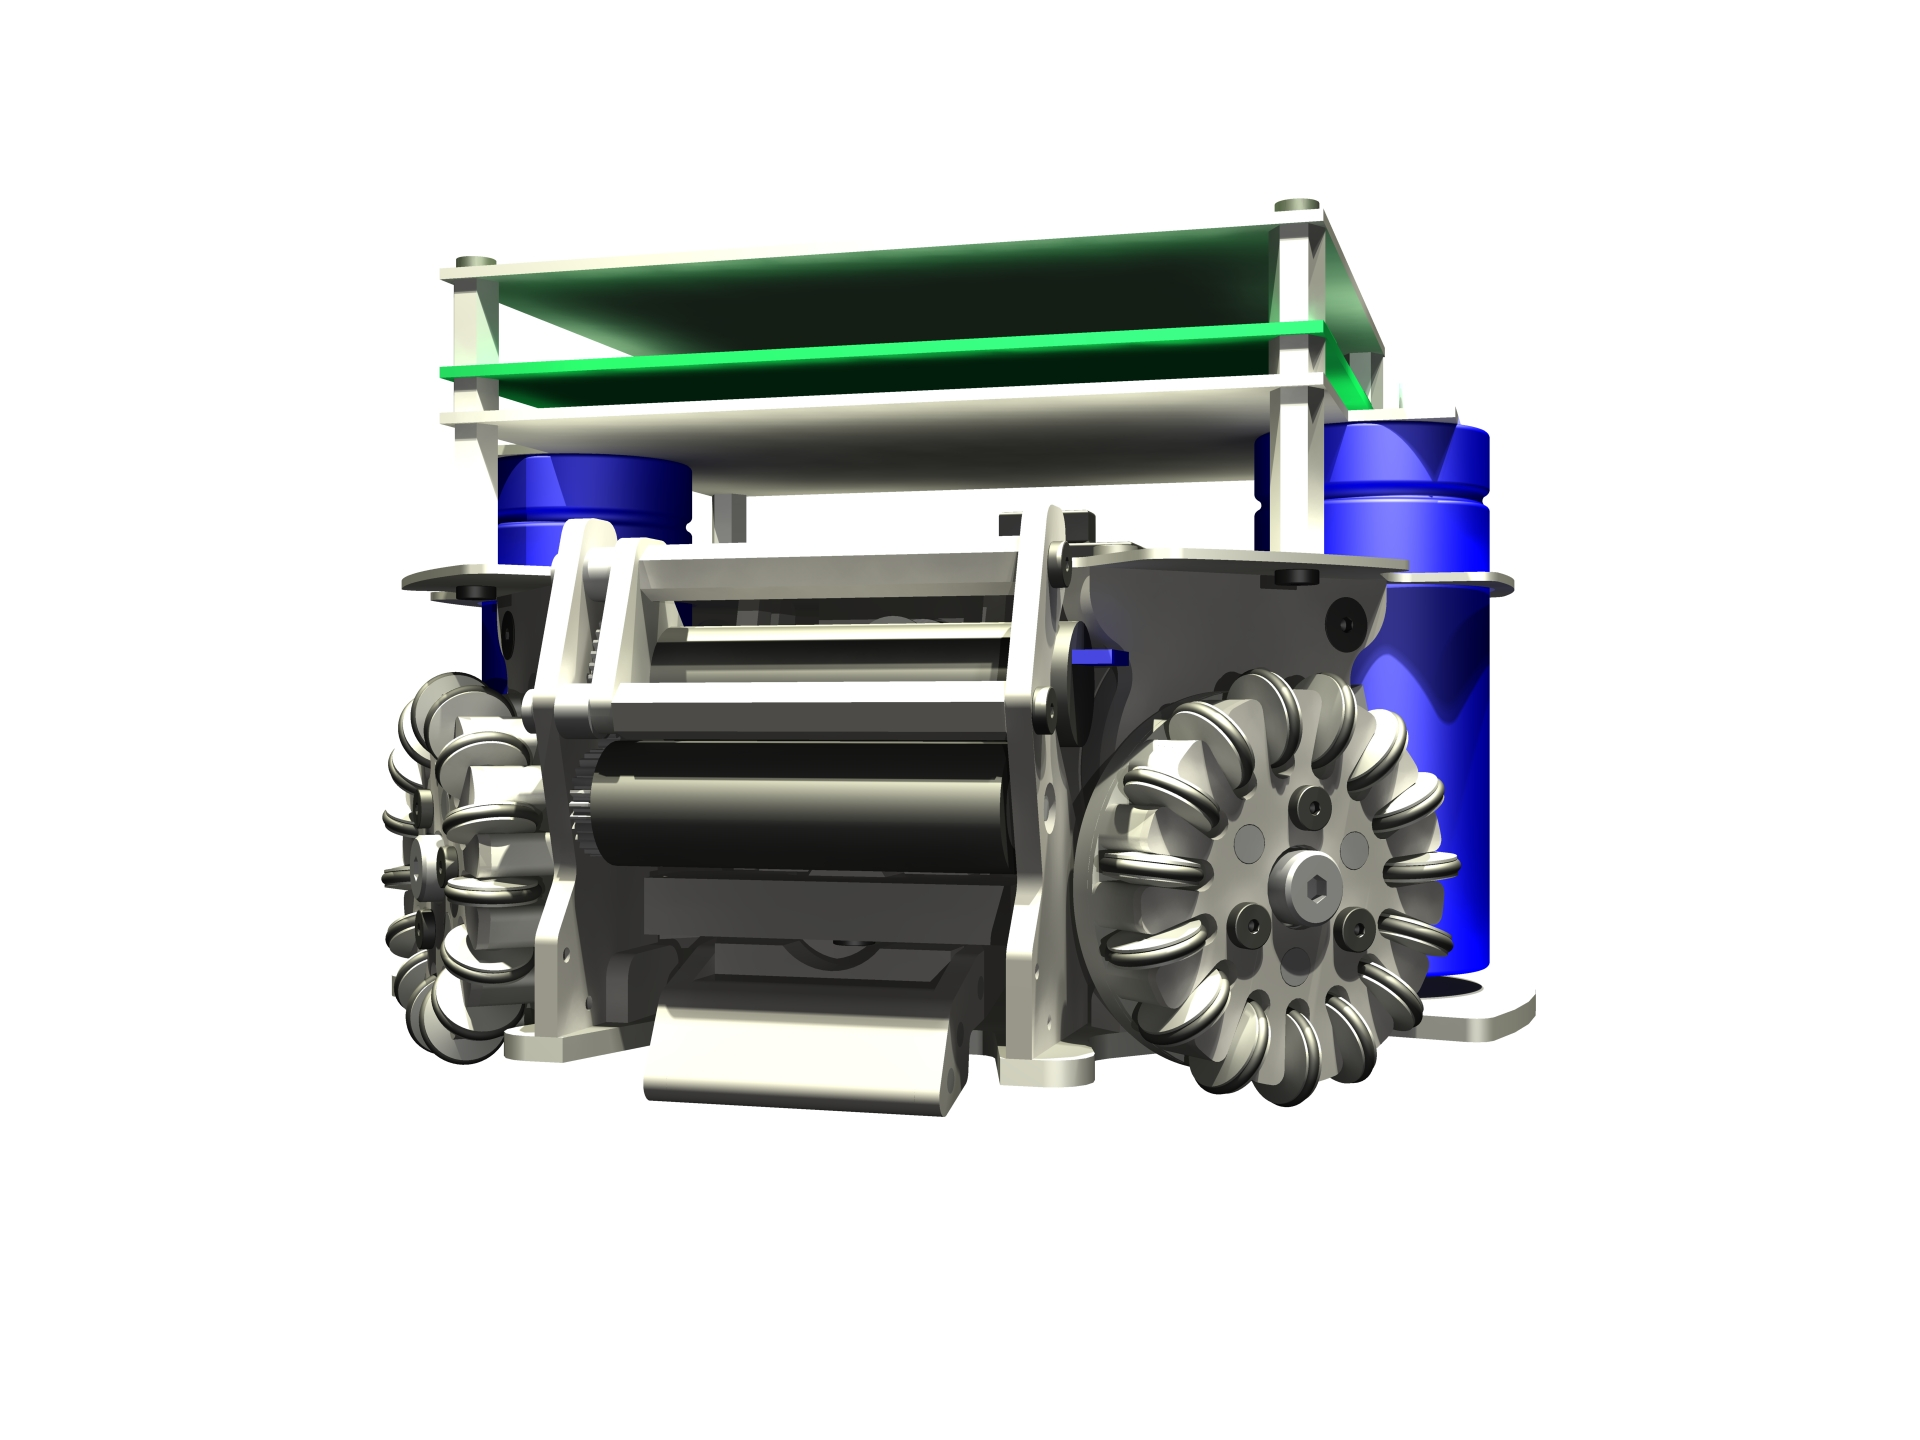
\includegraphics[width=0.3\textwidth]{images/2010Robot}
	\caption{2007 Robot (left) vs. 2008 Robot (center) vs. 2010 Robot CAD Rendering (right)}
	\label{fig:RobotComparison}
\end{figure}


\paragraph{}
% Has been updated. Refined by Andy, brain hurts, reread
While our previous robots participated successfully in spirited competition, we are developing a new team with increased capabilities for the 2010 season. In particular, the 2010 robots boast a chipper and wheel encoders. Lessons learned in competition and testing of the 2008 fleet motivated us to place special emphasis on increased manufacturability and reliability. Testing and validation of new components uses the previous systems as benchmarks for comparison and follows similar methods as those outlined in our 2008 Team Description Paper \cite{robocup08tdp}. The new team will be no larger than 179mm in diameter and 149mm tall.

\subsection{Reliability, Manufacturability, and Maintainability}
\paragraph{}
% Has been updated. And sustainability? Refined by Andy, reread
A number of improvements are planned to enhance manufacturability, reliability, and maintainability of the 2010 team. In 2008, due to extreme cost cutting, set screws were used, throughout the vehicles to attach gears to shafts. As expected, this became an unfortunate reliability concern. In the 2010 design, custom pinion shafts are used eliminating the need for set screws. In addition, the use of pinion shafts makes the drive train more compact leaving more room for ball manipulation apparatus.

\begin{figure} 
	\centering
	\vspace {0 cm}
	\includegraphics[width=0.3\textwidth]{images/Dribbler}
	\includegraphics[width=0.3\textwidth]{images/DriveModule}
	\includegraphics[width=0.3\textwidth]{images/DriveMotorModified}
	\caption{From right to left, (a) dribbler, (b) drive module, and (c) modified drive motor}
	\label{fig:SimplifiedAssembly}
\end{figure}

\paragraph{}
% Has been updated. Refined by Andy, reread
To further increase the reliability and maintainability of the new team, the drive modules are now held in place with two locating pins and a single screw on the bottom and one screw on the top. The dribbler is attached to the bottom plate with a similar screw and locating pin configuration. Both assemblies are shown in Figure \ref{fig:SimplifiedAssembly}. These changes have decreased the number of screws in each robot by over half and have increased the locational accuracy of all components.

\subsection{Omni Wheel}
\paragraph{}
% Has been updated. Updated by Andy
Our latest designs address a few key problems with the old omniwheel design. The previous designs suffered from excessive carpet fiber buildup which could be only mitigated by a complex cleaning procedure. In addition, refinements were made to accommodate the new drive modules.
\paragraph{}
% Has been updated. Updated by andy
To address carpet buildup, the edges of the rollers are now tapered. Additionally, the formerly sharp edges of the wheel bodies were filleted to provide a smoother interaction with the carpet. To simplify cleaning procedures the new fleet uses a small dowel pin as an axel for each roller. It should also be noted that the new rollers are compatible with both 2008 and 2010 wheel bodies.

\subsection{Drive Module}
\paragraph{}
% Has been updated. Refined by Andy
To make room for the chipper and wheel encoders, the drive modules had to be completely redesigned. Each assembly is composed of a single plate which supports both the motor and wheel and a plate to support the encoder. Just as in previous years, we use Maxon EC45 pancake brushless motors. The gear ratio was decreased slightly from 5:1 to 9:2 allowing for a slight increase in speed. In addition, the gear teeth were made much larger making the drive train less susceptible to fibers and and other foreign matter. This design change is achieved through an internal gear mounted to the rear of each omni wheel which mates with a custom pinion shaft installed in the motors. This shaft repaces the stock shaft and protrudes out the rear of the motor connecting to an encoder. A modified drive motor is shown in Figure \ref{fig:SimplifiedAssembly}. 

\subsection{Dribbler}
\paragraph{}
% Has been updated. Refined by Andy
The dribbler is the assembly which controls the ball during gameplay. The mechanism utilizes a custom steel pinion shaft covered with silicone rubber tubing to increase adhesion. Just as in 2008, a Maxon EC16 brushless motor mated to a GP16A planetary gearhead spins the dribbler shaft through a simple 1:1.4 gearbox. The use of ball bearings rather than bushings increase efficiency and a larger tooth size decreases susceptibility to foreign object contamination. Additionally, the assembly incorporates a break-beam ball sensor. The dribbler's ball coverage is no more than 19\%.

\subsection{Kicker}
\paragraph{}
The robot's kicker is the primary method of both scoring and passing. A solenoid is mounted inside the robot and a large amount of current is discharged into it from a capacitor bank. In order to accommodate a more powerful solenoid, large off-the-shelf solenoids have been purchased and have had their casing removed to fit dimensional restrictions. The changes will allow for more powerful kicks while still allowing the kicker system to fit within the same size restrictions. A more robust kicker boot has also been implemented which, unlike the 2008 kicker boot, is designed so that it does not bend under the large forces felt while kicking the ball. The kicker plunger will be made of a front aluminum component and a rear steel component. The use of aluminum reduces energy losses due to the solenoid's magnetic field pulling back on the plunger after it has been fired.

\subsection{Chipper}
\paragraph{}
The chipper allows the robots to pass the ball by chipping it into the air. It can shoot the ball over opponents and adds greater flexibility to planning algorithms while reducing chances of interception. The chipper boot is located underneath the kicker boot. When a robot is in possession of the ball, the dribbler rolls the ball up against the chipper boot. The chipper is powered by a solenoid which is mounted above the kicker solenoid. In order to transfer power from the solenoid to the chipper, two arms are used that act like levers. When the solenoid fires and pulls the plunger back, the arms rotate and move the chipper
boot forward, chipping the ball up. Currently two different chipper systems are being tested. The results will help determine the correct arm length, solenoid power, chipping angle. To reduce mechanical losses from friction, future chipper system designs will implement pancake solenoids which will fire in the same plane as the chipper boot, removing the need for any mechanical interface.

\section{Electrical}
The electronics system is broken into the following two broad subsystems:
\begin{description}
 \item[Controller Circuitry] contains the radio link to the computers on the sidelines, and all motor control functionality.
 \item[Kicker Circuitry]  drives the kicker and chipper solenoids.
\end{description}
In comparison to the previous design revision, we added a chipper solenoid, but the charger and other switching mechanisms have remained largely the same. 

\begin{figure}
       \centering
       \vspace {0 cm}
       \includegraphics[height=0.3\textwidth]{images/elec}
       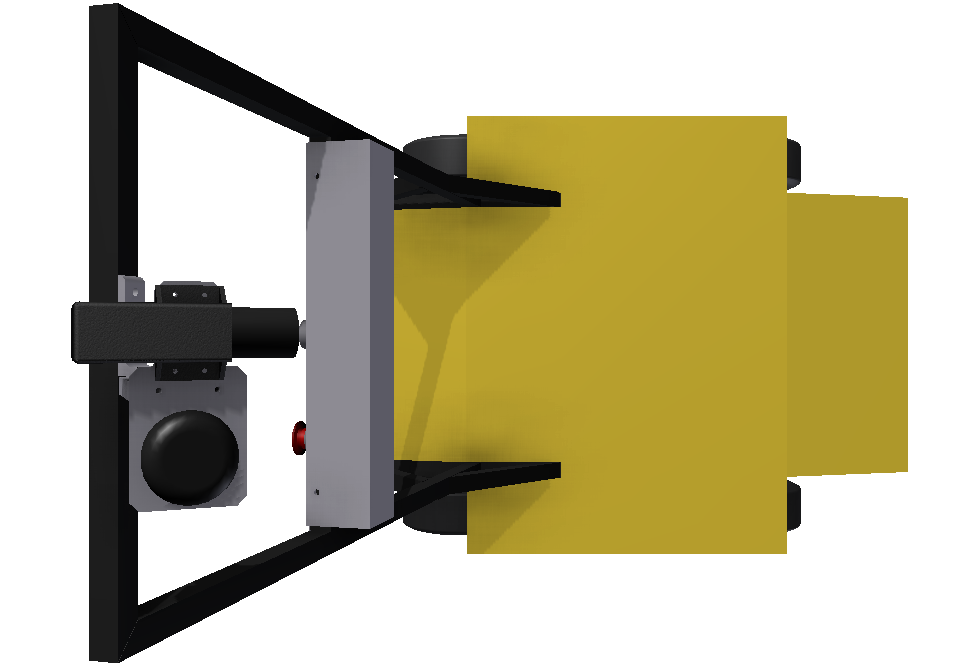
\includegraphics[height=0.3\textwidth]{images/top}
       \caption{Block diagram for the controller board (left), and a photograph of the actual board.}
\end{figure}

\subsection{Controller}
The primary functionality of the controller subsystem is to translate motor speeds sent by the computer on the sidelines to actual motor values. Though the controller is currently "dumb" we hope in the future to enable more intelligence on the robot.

The requirements of the electrical system derive from the requirements of the drive and dribbler motors. Each motor has three phases connected in a wye configuration and three hall effect sensors to establish rotor position. To drive a brushless motor the rotor position is used to determine which coils should be energized. A coil is energized with a half bridge. Each half bridge is composed of an N and P channel FET driven by a Microchip FET driver (TC4428). There are three half bridges per motor (one for each coil) for a total of 15 half bridges per robot. With miscellaneous passives, the motor driver circuitry composes about 150 components on each board. The half bridges are driven by a Xilinx 100K gate Spartan 3E (XC3S100E) FPGA. The FPGA is memory mapped to a NXP ARM7 (LPC2103) which handles local feedback control with information from US Digital encoders.

The robot communicates to the server via Texas Instruments CC1101 wireless ASSC. This ASSC allows tuning from 779MHz to 928MHz including the 868MHz ISM band. Packets from the radio modules are routed through the FPGA to the ARM to allow for future work in hardware accelerated wireless protocol research. Due to poor wireless performance in the previous year, and severe space constraints in the current design, standard monopole antennas were not used. Instead, a balanced dipole "halo" antenna will be utilized. The antenna is ideally suited for the challenge as it is very low profile and omnidirectional \cite{harrisonjr1961fda}.

In a typical design, power supplies and their distribution are normally considered a trivial implementation task. In contrast, this design has five power rails; 1V2, 1V8, 2V5, 3V3, and VBATT (12V). The many power rails present a considerable routing challenge. Despite this, the board is only two layers which affords much quicker and cheaper manufacturing then other processes. The 3V3 power supply is switching for high efficiency while the other lower voltages are produced with simple linear low dropout regulators.

\subsection{Kicker}
The kicker circuitry charges a bank of capacitors which are then discharged into the solenoids (both the kicker and the chipper) to kick the ball. The kicker uses a Linear Technologies LT3750 flyback controller to convert the battery voltage (12V) to approximately 250 volts which charges a 5400$\mu$F capacitor bank. The capacitors are discharged into the solenoids by means of an Insulated Gate Bipolar Transistor (IGBT). Ball speeds approaching legal limit have been achieved. In comparison to other designs, this design is quite compact, requiring only about three square inches of board area. This design also boasts efficiencies exceeding 80\%. 


\section{Conclusion}
For the 2010 season, we intend to have a new fleet of robots incorporating the lessons learned through the last design revision, as well as an improved robust passing and control system.  This should allow both significantly faster and more competitive gameplay, as well as more reliable robots with fewer maintenance requirements.  

\bibliographystyle{splncs}
\bibliography{references}

\end{document}
